\phantomsection
\setsection{BUỔI 3-4: CÀI ĐẶT VÀ TRIỂN KHAI VUE}
\setcounter{section}{1}
% =========================================================
% \clearpage
\phantomsection
\setsubsection{Bước 1: Tạo ứng dụng Vue}
\setcounter{subsection}{1}
\setcounter{figure}{0}
\begin{figure}[H]
    \centering
    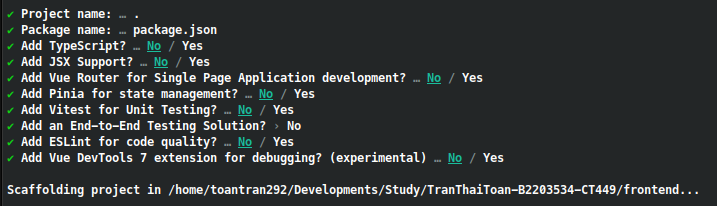
\includegraphics[width=15cm]{imgs/1.png}
    \caption{\bfseries Tạo ứng dụng Vue}
\end{figure}
\begin{figure}[H]
    \centering
    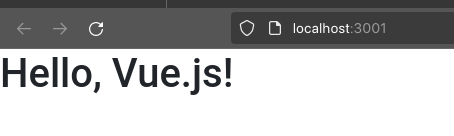
\includegraphics[width=15cm]{imgs/2.png}
    \caption{\bfseries Kết quả sau khi chạy Vue}
\end{figure}
% =========================================================

\phantomsection
\setsubsection{Bước 1: Quản lý mã nguồn dự án với Git và Github}
\setcounter{subsection}{1}
\setcounter{figure}{0}
\begin{figure}[H]
    \centering
    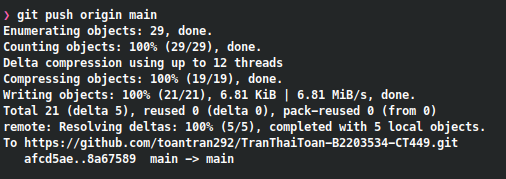
\includegraphics{imgs/4.png}
    \caption{\bfseries Push code lên github}
\end{figure}

% =========================================================
\phantomsection
\setsubsection{Bước 3: Cài đặt trang hiển thị danh sách các liên hệ}
\setcounter{subsection}{3}
\setcounter{figure}{0}
\begin{figure}[H]
    \centering
    
\includegraphics[width=15cm]{imgs/3.png}
    \caption{\bfseries Giao diện trang danh sách}
\end{figure}
% =========================================================
\phantomsection
\setsubsection{Bước 4: Tạo trang lỗi 404 không tìm thấy trang}
\setcounter{subsection}{4}
\setcounter{figure}{0}
\begin{figure}[H]
    \centering
    
\includegraphics[width=15cm]{imgs/5.png}
    \caption{\bfseries Giao diện trang 404 Not Found}
\end{figure}
\begin{figure}[H]
    \centering
    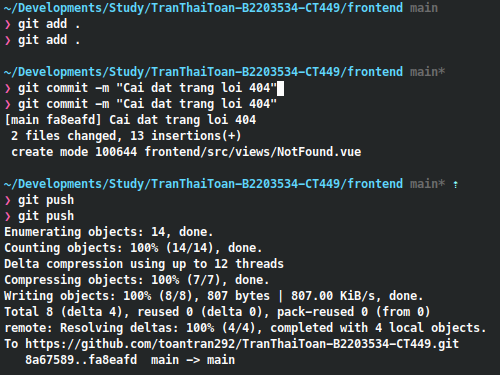
\includegraphics{imgs/6.png}
    \caption{\bfseries Push code trang 404 lên github}
\end{figure}
% \begin{figure}[H]
%     \centering
%     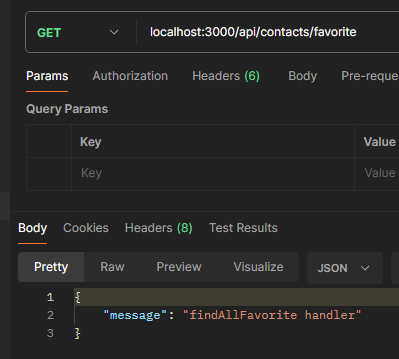
\includegraphics{imgs/14.png}
%     \caption{\bfseries Thử API find all contact favorites bằng postman}
% \end{figure}
% \begin{figure}[H]
%     \centering
%     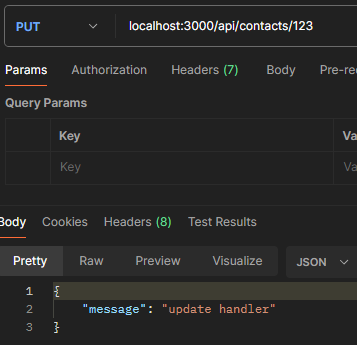
\includegraphics{imgs/15.png}
%     \caption{\bfseries Thử API update contact favorites bằng postman}
% \end{figure}
% =========================================================
\phantomsection
\setsubsection{Bước 5: Tạo trang cập nhật liên hệ}
\setcounter{subsection}{5}
\setcounter{figure}{0}
\begin{figure}[H]
    \centering
    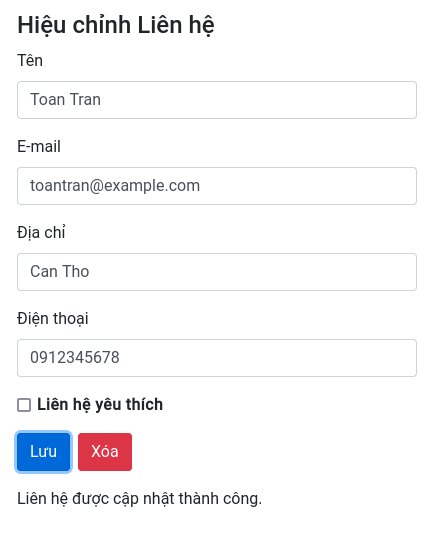
\includegraphics{imgs/7.png}
    \caption{\bfseries Trang cập nhật liên hệ}
\end{figure}
\begin{figure}[H]
    \centering
    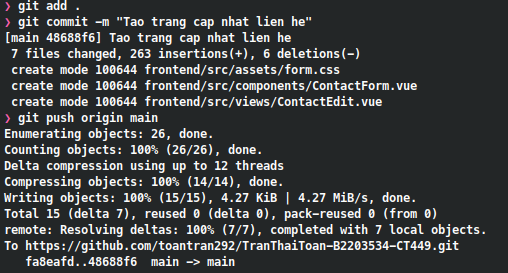
\includegraphics{imgs/8.png}
    \caption{\bfseries Push code trang cập nhật liên hệ lên github}
\end{figure}
% =========================================================
\phantomsection
\setsubsection{Bước 6: Tạo trang thêm liên hệ}
\setcounter{subsection}{5}
\setcounter{figure}{0}
\begin{figure}[H]
    \centering
    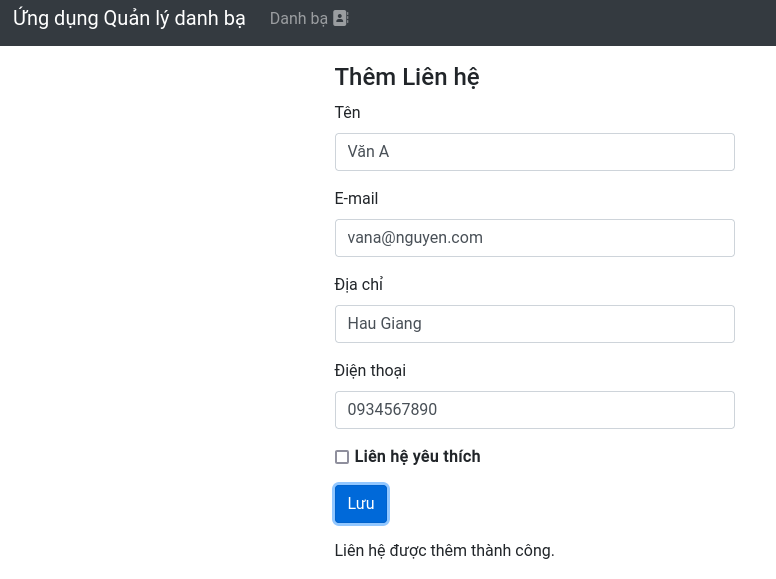
\includegraphics[width=15cm]{imgs/9.png}
    \caption{\bfseries Trang thêm liên hệ}
\end{figure}
\begin{figure}[H]
    \centering
    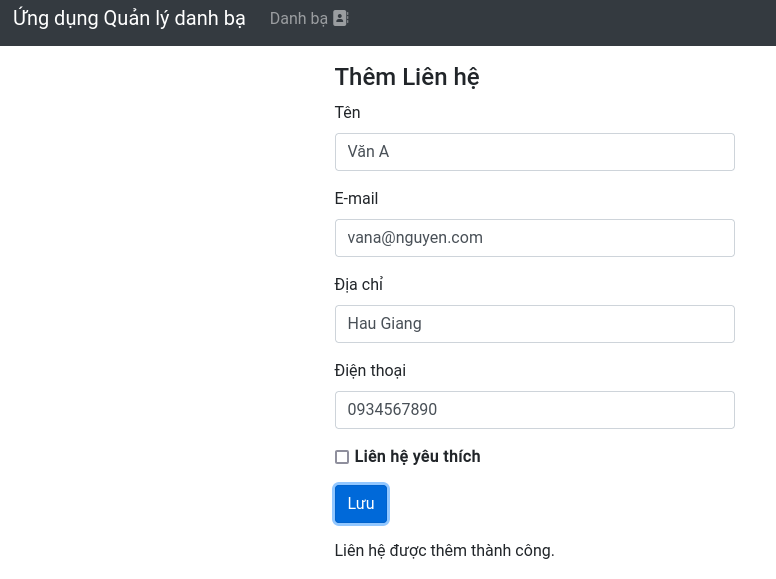
\includegraphics[width=15cm]{imgs/9.png}
    \caption{\bfseries Trang danh sách sau khi thêm liên hệ}
\end{figure}